% Diese Zeile bitte -nicht- aendern.
\documentclass[course=erap]{aspdoc}
\usepackage{graphicx,amsmath,amssymb}
\usepackage{parskip}
\usepackage{pgfplots}
\usepackage{hyperref}
\graphicspath{ {./images/} }
%%%%%%%%%%%%%%%%%%%%%%%%%%%%%%%%%
%% TODO: Ersetzen Sie in den folgenden Zeilen die entsprechenden -Texte-
%% mit den richtigen Werten.
\newcommand{\theGroup}{143} % Beispiel: 42
\newcommand{\theNumber}{A208} % Beispiel: A123
\author{Ar Pazari \and Edera Ndoj \and Demil Omerovic}
\date{Wintersemester 2023/24} % Beispiel: Wintersemester 2019/20
%%%%%%%%%%%%%%%%%%%%%%%%%%%%%%%%%

% Diese Zeile bitte -nicht- aendern.
\title{Gruppe \theGroup{} -- Abgabe zu Aufgabe \theNumber}

\begin{document}
\maketitle
\section{Einleitung}
Ein wichtiger
Algorithmus im Bereich der Bildverarbeitung ist die Gamma-Korrektur, die die Anpassung von Helligkeit und Kontraste in digitalen Bildern ermöglicht\cite{GammaKorr}. 
Unsere Aufgabe umfasste die eingehende Untersuchung dieses Algorithmus, sowohl in der theoretischen  als auch in der praktischen Betrachtung, um ihn in verschiedenen Implementierungen praktisch umzusetzen. 

\begin{figure}[h]
\centering
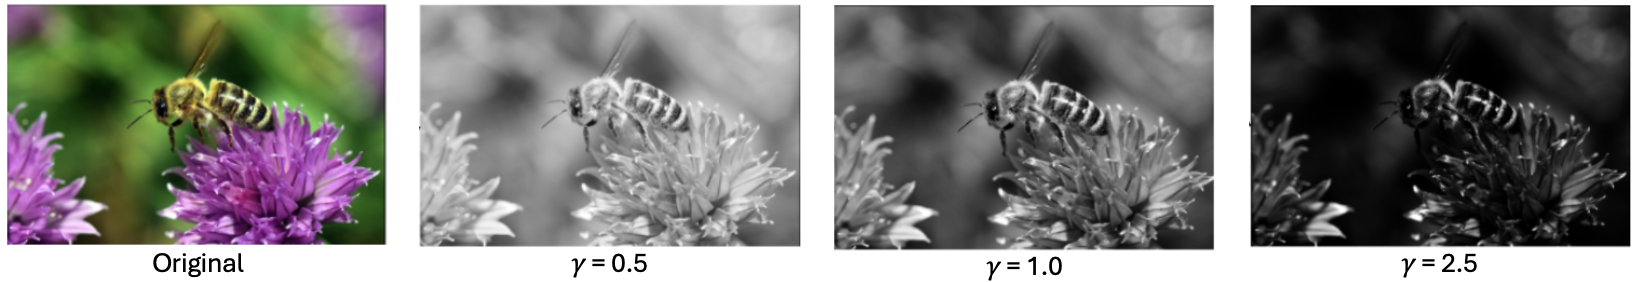
\includegraphics[width = 1\textwidth]{images/gamma1.png}
\caption{Visualisierung des Algorithmus}
\label{fig:1}
\end{figure}

\subsection{Funktionsweise des Algorithmus}
Die Bestandteile der Funktionsweise unseres Projektes werden schrittweise erklärt:
$P(x,y)$ repräsentiert vektorenweise ein Farbpixel an der Position $(x,y)$ im Bild $P$, wobei die RGB-Werte zur Darstellung dienen. Der Bildbereich ist durch $D = \{0, \ldots, \text{Breite} - 1\} \times \{0, \ldots, \text{Höhe} - 1\}$ definiert, wobei jedes Pixel seine Dimensionen einnimmt. \par

\textbf{1.} Das erste Berechnungsschritt ist die Umwaldung in Graustufen\cite{Graust}. Es erfolgt durch einen gewichteten pixelsweise Durchschnitt: 
\begin{equation}
D = \frac{a \cdot R + b \cdot G + c \cdot B} {a + b + c} \label{eq: gamma_correction_1}, 
\end{equation}
wobei $R, G, B$ die drei Farbkanäle Rot, Grün und Blau repräsentieren. Für die Koeffizienten $a, b, c$ werden üblicherweise die folgenden Werte verwendet: 
\begin{center}
\(a = 0.299\), \(b = 0.587\) und \(c = 0.114\).\par
\end{center}
Grund, warum die oben definierten Werte häufig verwendetet sind, liegt in der menschlichen Wahrnehmung von Farben und Helligkeit\cite{ColWahr2} und die Eigenschaften des Menschlichen Visuellen Systems (HVS)\cite{ColWahr1}. Diese Koeffizienten basieren auf der Empfindlichkeit des menschlichen Auges gegenüber verschiedenen Farben, wobei Rot (R) etwa 30\% zur Helligkeit beiträgt, Grün (G) etwa 59\% und Blau (B) etwa 11\%. \par
\begin{table}[ht]
\centering
\begin{tabular}{|l|c|c|c|c|}
\hline
Methode / Standard & Rot (R) & Grün (G) & Blau (B) & Gamma \\
\hline
ITU-R BT.601-7 (SDTV) & 0.299 & 0.587 & 0.114 & 2.2 \\
ITU-R BT.709-6 (HDTV) & 0.2126 & 0.7152 & 0.0722 & 2.2 \\
ITU-R BT.2020 (UHDTV) & 0.2627 & 0.6780 & 0.0593 & 2.4 \\
Digitale Fotografie & 0.3 & 0.59 & 0.11 & 2.2 \\
Gleichmäßige Gewichtung (Einfach) & 0.333 & 0.333 & 0.333 & 2.2 \\
\hline
\end{tabular}
\caption{Koeffizienten und Gamma-Werte für die Graustufenkonvertierung\cite{ITU_INT}}
\label{tab:grayscale_conversion}
\end{table}
\textbf{2.} Das Ergebnis des ersten Schrittes ist der einzelne Intensitätswert D, der die Helligkeit dieses Pixels darstellt:
\begin{equation}
Q_(x,y) = D
\end{equation} 
\textbf{3.} Anschließend unterzieht sich das Graustufenbild einer Gammakorrektur:
\begin{equation}
Q'_(x,y) = \left(\frac{Q_(x,y)}{255}\right)^\gamma \cdot 255 \label{eq: gamma_correction}
\end{equation}
wobei $\gamma \in [0, \infty)$ eine vom Benutzer festgelegte Fließkommazahl ist. Wenn $\gamma < 1$ erscheint die Ausgabedatei heller; bei $\gamma > 1$ wird sie dunkler. Wenn $\gamma = 1$ werden die ursprünglichen Pixelwerte unverändert\cite{GammaGraphik}. Der am häufigsten verwendete $\gamma$-Wert ist $2.2$. Es hilft, die Anzeige von Bildern auf Geräten wie z.B Monitoren zu korrigieren, die in der Regel eine nicht lineare Reaktion auf Intensitätsstufen aufweisen. Diese Wahl resultiert aus historischen Standard \cite{DigBildVer}.\par

\begin{figure}[ht]
\centering
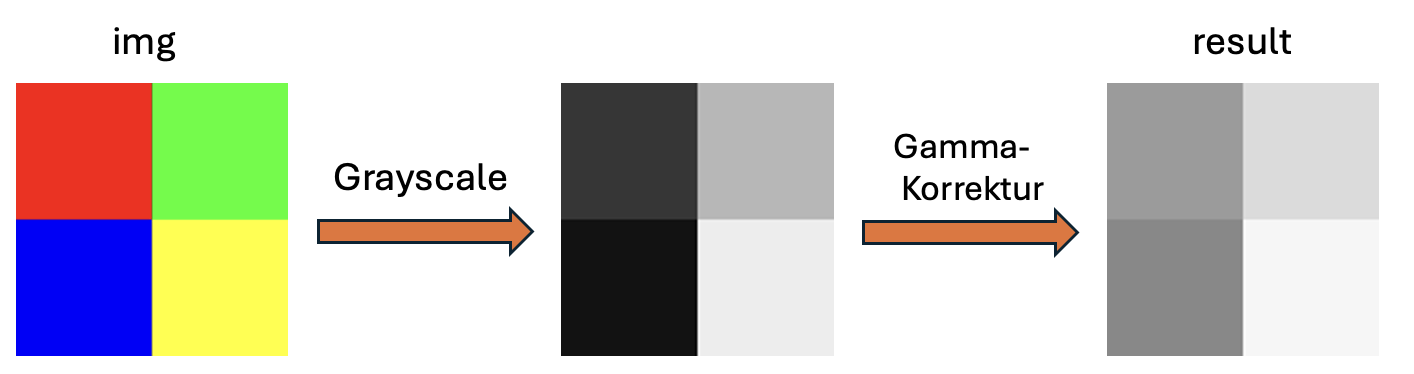
\includegraphics[width =0.65\textwidth]{explanation.png}
\caption{Visualisierung des Algorithmus}
\label{fig:2}
\end{figure}

Nach den beiden Schritten besteht die Ausgabedatei aus Pixeln, deren Intensitätsinformationen von Schwarz bis Weiß abhängig von das Gammawert variieren. 
\subsubsection{Die Eingabedatei}
\textbf{Die Eingabedatei} ist keine Textdatei, sondern ein \textbf{24bpp PPM (P6) Bilder}\cite{P6Files}. Die Benutzung von P6 PPM Dateien ermöglicht eine einfache und klare Darstellung von Farbinformationen. Die Bestandteile einer P6 Eingabedatei sind:\\
-\textbf{Magischer Wert}: Identifiziert das Format der PPM Bilder (hier: "P6", codiert in ASCII)\\
-\textbf{Breite und Höhe des Bilds} (codiert in ASCII)\\
-\textbf{Maximalwert des Farbwertes} (codiert in ASCII) \\
-\textbf{Die Werte der Pixel}, die binär codiert werden, erhalten jeweils drei Bytes für die Farkanäle $R, G, B$. Mit 24 Bits pro Pixel beträgt die maximale Anzahl von darstellbaren Farben $2^{24}$, was $16.777.216$ Farben entspricht. Diese umfassende Farbpalette ermöglicht die Darstellung von detailreichen Bildern.

% \begin{figure}[h]
% \centering
% 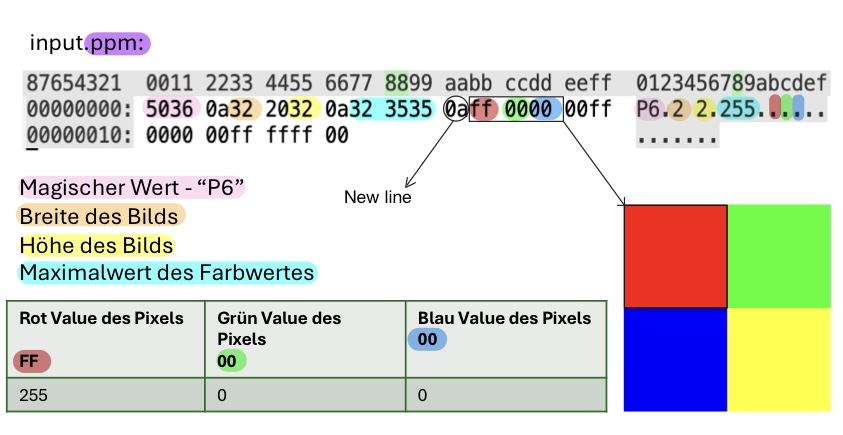
\includegraphics[width =0.75\textwidth]{input_example.jpg}
% \caption{Visualisierung der Eingabedatei des Formats P6 PPM}
% \label{fig:3}
% \end{figure}

\subsubsection{Die Ausgabedatei}
\textbf{Die Ausgabedatei} sollte in ein effizientere \textbf{Netpbm-Format} repräsentiert sein. Der Wechsel von (P6) Input Format zielt darauf ab, die Dateigröße zu reduzieren und die Repräsentation der Ausgabedatein zu vereinfachen.
Da die Resultät ein Graustufenbild ist und eine geringere Dateigröße hat, wurde die Nutzung von \textbf{P5 PGM (Portable Graymap Format)}\cite{P5Files} Dateien die Interpretation des Pixels erleichtern. Im Gegensatz zu P6 Dateien, es wird nur ein Byte benötigt, um die Intensitätsinformationen jedes Pixels zu speichern. Deswegen wurde die Dateigröße um zwei Drittel reduziert, was zu einer effizienteren Speicherung führt. Als Binärdateiformat ist P5 auch nicht lesbar für Menschen, aber das Lesen und Schreiben Operationen sind im allgemeinen schneller. Eine andere PGM Format ist \textbf{P2}\cite{P2Files}, welches nur eine begrenzte Anzahl von Graustufen ermöglicht und somit nicht die notwendige Genauigkeit für die Gamma-Korrektur bietet. Deswegen wurde \textbf{P5} gewählt, um eine präzisere Repräsentation der Bildinformation sicherzustellen.\par
Die Bestandteile einer P5 Ausgabedatei sind:\\
-\textbf{Magischer Wert}: Identifiziert das Format der PGM Bilder (hier: "P5", codiert in ASCII)\\
-\textbf{Breite und Höhe des Bilds} (codiert in ASCII decimal)\\
-\textbf{Maximalwert des Farbwertes} (codiert in ASCII decimal: Hier 255, da die initiale Pixels als $uint8$ dargestellt sind. Daher reicht der Bereich 0-255, um die Helligkeitsstufen der korrigierten Pixel effizient zu repräsentieren.) \\
-\textbf{Die Werte der Pixel}, die binär codiert werden, erhalten jeweils ein Byte für  deren Intensitätsinformationen.  

% \begin{figure}[h]
% \centering
% 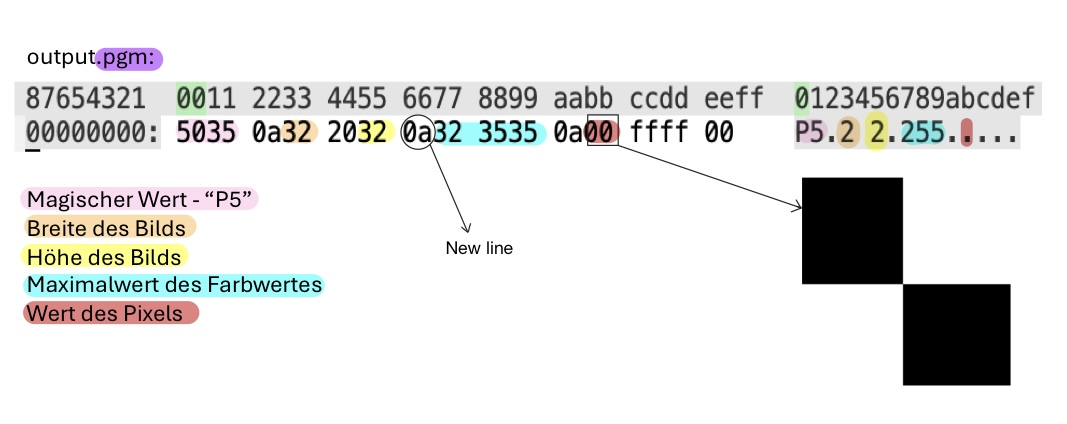
\includegraphics[width =0.75\textwidth]{output_example.jpg}
% \caption{Visualisierung der Ausgabedatei des Formats P5 PGM}
% \label{fig:4}
% \end{figure}

\subsubsection{Exponentialfunktion mittels grundlegender mathematischer Operationen}
Eine weitere Herausforderung ist eine Möglichkeit zu finden, die die in dritter Formel angewendete Exponentialfunktion \eqref{eq: gamma_correction} nur mittels grundlegender mathematischer Operationen zu berechnen. \textbf{Unter Verwendung der babylonischen Methode} \cite{BabylMeth} bzw. Herons Methode kann man die Exponentialfunktion ersetzen wie folgt:
\begin{equation}
    x_{n+1} = \frac{1}{2} \left( x_n + \frac{a}{x_n} \right),  \quad n \in \mathbb{N} \label{eq: bab_meth}
\end{equation}
wobei $x_n$ die Anfangsvermutung (z.B die Zahl oder die Hälfte der Zahl, deren Quadratwurzel gesucht wird). $a$ ist die Zahl, deren Quadratwurzel bestimmt werden soll. Die sukzessiven Näherungen $x_n+1$ werden gemäß der oben definierten Iterationsschritte berechnet. Diese Formel wird so lange wiederholt, bis der Prozess konvergiert, also bis ein konsistentes sowie klar definiertes Ergebnis erreicht wird. Eine zehnmalige Wiederholung der Iterationsschritt ergibt eine gute Annäherung an die Quadratwurzel. \par
Eine andere Möglichkeit ist \textbf{die Taylor Reihe} \cite{TaylorReih}. Für die Berechnung von \(a^b\) verwenden wir die Taylor Reihe für die Exponentionalfunktion: 
 \begin{equation}
    e^x = 1 + x + \frac{x^2}{2!} + \frac{x^3}{3!} + \ldots \label{eq:Taylor-Reihe}
\end{equation}

Hier wurde \(a^b\) als \(e^{b \cdot \ln(a)}\) approximiert, wobei \(\ln(1+x) \approx x - \frac{x^2}{2} + \frac{x^3}{3} - \ldots\) den natürlichen Logarithmus approximiert. Diese Methode ermöglicht eine ungefähre Berechnung von  \(a^b\) unter Verwendung einer endlichen Anzahl von Termen, was die Komplexität reduziert. 

\section{Lösungsansatz}
Implementiert wurde der Gamma-Korrektur Algorithmus auf 5 verschiedene Weisen, die sich alle in den unten detaillierten Ansätze widerspiegeln werden. Sie unterscheiden sich hinsichtlich Optimierungen, mathematischer Vorgehensweise und Reihenfolge der Datenverarbeitung und Zwischentransformationen voneinander.  
\subsection{Implementierung 1: Exponentialfunktion durch math.h}
Die erste Implementierung, dass \texttt{gamma\_V0.c} heißt, wurde mit den Methoden aus der Mathematikbibliothek (\texttt{math.h}) zur Berechnung der Exponentialfunktion umgesetzt. Das Pixelarray eines Eingabebildes wurde durchläuft und für jedes Pixel den Gamma Korrekturalgorithmus angewendet wurde. Zuerst erfolgt eine Umwandlung in Graustufen, indem die RGB-Farbwerte jedes Pixels entsprechend den gegebenen Koeffizienten a, b und c gewichtet werden. Anschließend wird die Gamma Korrektur durchgeführt, wobei die Exponentialfunktion aus der \texttt{math.h}-Bibliothek verwendet wird. 

\begin{figure}[h]
\centering
\includegraphics[width =0.65\textwidth]{images/gamma_v0.png}
\caption{Visualisierung einer Beispielverwendung der \texttt{gamma\_V0.c}}
\label{fig:3}
\end{figure}

Die ausgewählte Funktion \texttt{pow()} minimiert mögliche Rundungsfehler, die bei Fließkommazahlen auftreten können. Das Ergebnis wird auf den Bereich von 0 bis 255 begrenzt, um gültige Pixelwerte zu erhalten. Die resultierenden Pixelwerte werden im Ergebnisarray gespeichert, um die bearbeitete Ausgabedatei zu rekonstruieren. Die oben genannte Operationen wurden in die Funktion \texttt{gamma\_V0} implementiert. 



\subsection{Implementierung 2: Exponentialfunktion durch grundlegender mathematischer Operationen}
In der zweiten Implementierung, namens \texttt{gamma\_V1.c}, wurde der Algorithmus mithilfe der grundlegenden mathematischen Operatoren und zwei Hilfsfunktionen realisiert. 
Die erste Hilfsfunktion, \texttt{double integerPower(double base, int exponent)},
multipliziert die Basis mit sich selbst entsprechend dem ganzzahligen Exponenten (Vorkommastellen), während die zweite, \texttt{double fractionalPower(double base, double fractionalPart)}, die lineare Interpolation \eqref{eq: lineare_interpolation} und die Babylonische Methode \eqref{eq: bab_meth} für nicht-ganzzahlige Exponenten (Nachkommastellen) anwendet. Die Wahl zwischen Interpolation und Babylonische Methode für nicht-ganzzahlige Exponenten hängt davon ab, ob der \texttt{fractionalPart} kleiner oder größer $0.5$ ist. \par

\begin{figure}[h]
\centering
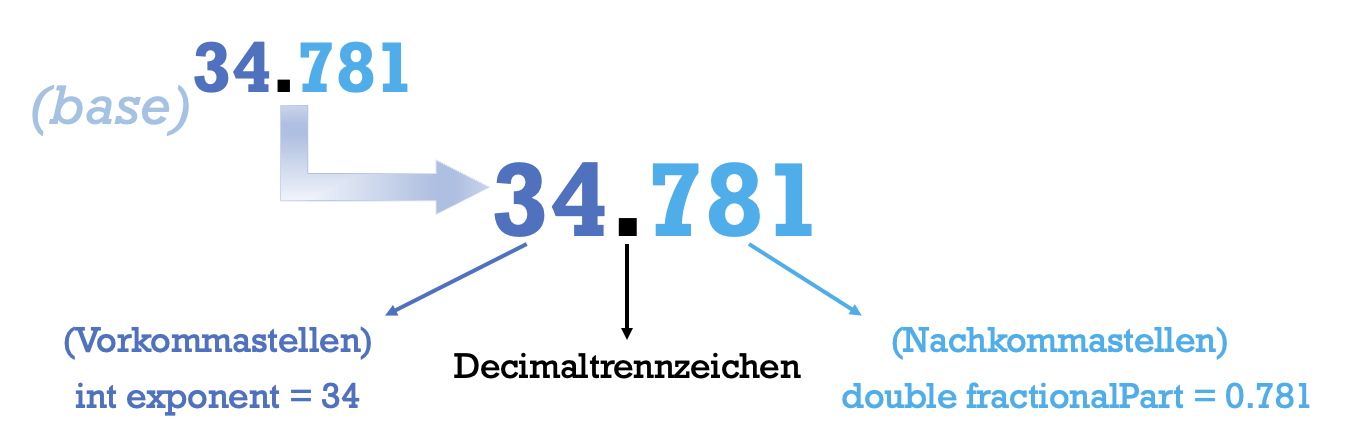
\includegraphics[width =0.65\textwidth]{nr_photo.png}
\caption{Die Trennung der $\gamma$-Wert in zwei Argumente für die Hilfsfunktionen}
\label{fig:4}
\end{figure}

Für die \texttt{fractionalPart} Werte kleiner als 0.5, erfolgt die Interpolation nach der Formel:
\begin{equation}
    1 + fractionalPart * (base - 1). \label{eq: lineare_interpolation}
\end{equation}
Die Formel\eqref{eq: lineare_interpolation} entspricht einer linearen Interpolation zwischen 1 (dem Ergebnis für eine Potenz von 0) und der Basis selbst (dem Ergebnis für eine Potenz von 1). Das ermöglicht eine glatte Übergangsberechnung wenn  \texttt{fractionalPart} nahe bei 0 liegt. Wenn es jedoch 0.5 oder größer ist, wird die Babylonische Methode\cite{BabylMeth} zur Berechnung der Quadratwurzel verwendet. Schließlich wurde eine andere Funktion namens \texttt{power} implementiert, die die Hilfsfunktionen aufruft, um das Ergebnis der Exponentialsfunktion zu berechnen, ohne die in \texttt{math.h} inklusierte \texttt{pow} Funktionen zu verwenden. Hier wurde das Exponent in 2 Teilen getrennt: \texttt{int exponent} und \texttt{double fractionalPart} und genutzt als Parametern in beide Hilfsfunktionen. Die Iteration durch das Pixelarray und die Transformationen erfolgen ähnlich wie in der ersten Implementierung in einer Funktion namens \texttt{gamma\_V1}. 
Insgesamt bietet diese Implementierung eine präzise Anwendung der Gamma-Korrektur und Flexibilität, die Berechnung der Exponentialfunktion ohne externe Bibliotheken durchzuführen. 

\subsection{Implementierung 3: Trennung der zweiten Haupttransformationen}
Um die Anforderungen der Aufgabestellung vollständig zu erfüllen, ist es notwendig, eine andere Implementierung zu realisieren, welcher ein Bild erst in Graustufen total konvertiert und anschließend eine Gammakorrektur auf allen Pixeln ausführt.
In \texttt{gamma\_V2.c} sind zwei Funktionen vorhanden, die die Transformationen der Farbpixel getrennt voneinander durchgeführen. Die Graustufenkonvertierung erfolgt durch die Funktion \texttt{convertToGrayscale()}, während die Gamma-Korrektur durch \texttt{applyGammaCorrection()} durchgeführt wird. 
Im Unterschied zu den vorherigen Implementierungen wird in dieser Version die Exponentialfunktion durch die Funktionen \texttt{exp} und \texttt{log} aus der \texttt{math.h}-Bibliothek ersetzt. Die Formel\eqref{eq: gamma_correction} wurde dann so aussehen:\\
\begin{equation}
Q'_(x,y) = \exp\left(\log\left(\frac{Q_{(x,y)}}{255}\right) \cdot \gamma\right) \cdot 255 
\end{equation}

Abgesehen von diesen gibt es noch eine weitere Methode namens \texttt{gamma\_V2()}, die nur die beiden Hilfsmethoden nacheinander anruft.
Der Parameter \texttt{img} von \texttt{gamma\_V2()}  ist auch der Eingabeparameter für \texttt{convertToGrayscale()}, das eine PPM-Datei nimmt und die Grauskalierungstransformation durchführt, um \texttt{first\_img} zu erstellen. Anschließend wird \texttt{first\_img} von der Funktion \texttt{applyGammaCorrection} verwendet, um für jedes Pixel eine Gamma-Korrektur durchzuführen, was schließlich zur endgültigen Ausgabe \texttt{result} führt. Eine detallierte Darstellung (siehe Abbildung \ref{fig:5}) der Funktionsweise der \texttt{gamma\_V2.c} ist hilfreich, um zu verstehen, in welche Aspekten \texttt{gamma\_V2.c} sich von den ersten Ansätzen unterscheidet. 

\begin{figure}[h]
\centering
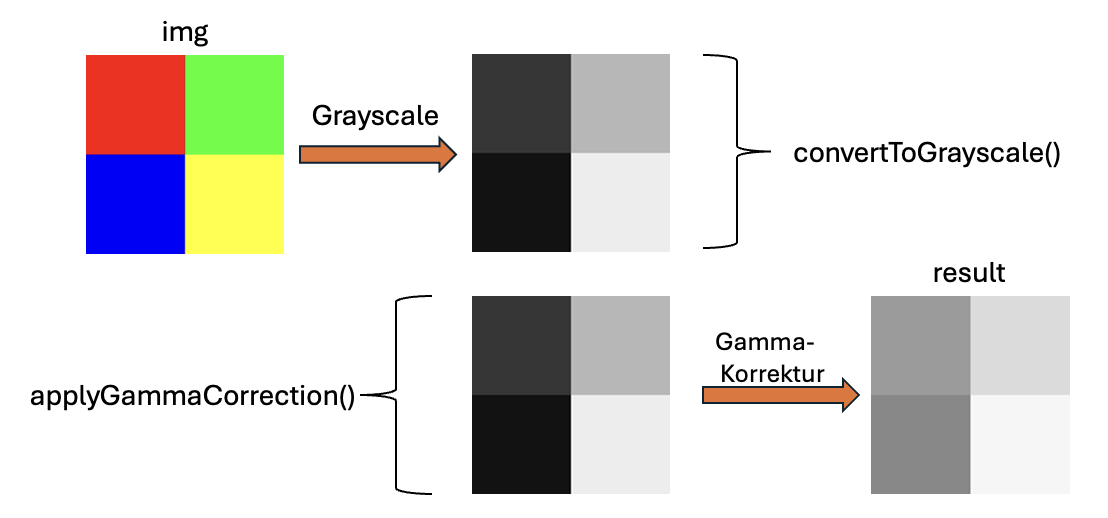
\includegraphics[width = 0.75\textwidth]{explanation_2.png}
\caption{Visualisierung der Funktion in \texttt{gamma\_V2.c}}
\label{fig:5}
\end{figure}
In dieser Implementierung sind die Transformationsschritte klar voneinander getrennt, und die Verwendung von \texttt{exp} und \texttt{log} stellt eine andere mathematische Herangehensweise dar. 

\subsection{Implementierung 4: Hybrider Ansatz - Kombination von SIMD und skalaren Operationen }

Die vierte Implementierung zielt darauf ab, die Verarbeitung von RGB-Bilddaten durch die Nutzung der SIMD-Befehlssätze weiter zu optimieren, wobei ein spezieller Fokus auf die effiziente Anordnung von Pixelwerten und die Kombination von SIMD- und Skalarberechnungen liegt. Im ersten Schritt werden die RGB-Pixelwerte als Integervariablen eingelesen und dann so neu ausgerichtet, dass in einer SIMD-Variablen mit 128 Bits vier rote, vier grüne und vier blaue Werte sequenziell gespeichert werden (siehe Abbildung \ref{fig:6}). 
Die restliche 1.3 Byte werden zwar geladen und mit berechnet aber sie werden im letzten Schritt nicht gespeichert. Sie werden in der darauffolgenden Iteration behandelt.

Trotz der Einschränkung, dass nur 5,3 RGB-Pixel in eine 128-Bit-Variable passen, ermöglicht diese Konfiguration eine effiziente Verarbeitung. 
Dabei werden die RGB-Werte zunächst in ein \texttt{\_\_m128i}-Variable geladen. Anschließend erfolgt eine Konvertierung von \texttt{\_\_m128i} zu \texttt{\_\_m128} (float), um die Berechnungen für die Graustufenkonvertierung in SIMD durchzuführen. Da die vorhandenen SIMD-Bibliotheken wie Intels SSE (Streaming SIMD Extensions)\cite{SEE} keinen spezifischen Befehl \textit{pow}-Funktion bieten, erfolgt die Berechnung der Gammakorrektur skalar.
Ein wichtiger Aspekt ist das Alignment der Daten. Die Entscheidung, die Daten auf 4 Bytes auszurichten und nicht auf 5, resultiert aus der Überlegung, dass bei einer Breite, die nicht durch 5 teilbar ist, in jeder Zeile vier skalare Berechnungen notwendig wären. Durch die Anordnung in 4-Byte-Blöcken reduziert sich die Anzahl der erforderlichen Skalarberechnungen auf drei, was zu einer effizienteren Verarbeitung führt.

\begin{figure}[h]
\centering
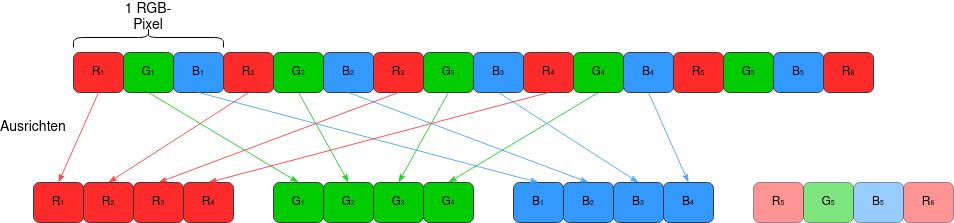
\includegraphics[width = 0.8\textwidth]{images/SIMD Diagramm.png}
\caption{Neuausrichtung der einzelnen RBG-Pixel}
\label{fig:6}
\end{figure}

\subsection{Implementierung 5: Optimierung - SIMD mit Approximationsfunktionen}
Dieser Ansatz ist aufbauend auf dem vorherigen, nur mit der Unterscheidung, dass anstatt teilsakalarer nun vollständige SIMD Berechnungen durchgeführt werden. Ein wesentlicher Unterschied ist, das dies hier mit Hilfe von Approximationsfunktionen innerhalb des SIMD-Frameworks erreicht wurde. 
Durch diesen Ansatz ergibt sich ein signifikanter Unterschied zu dem bereits beschriebenen Ansatz (\textit{2.4}), um die Gamma-Korrektur $x^{\gamma}$, effizienter durchzuführen.
Die Potenzfunktion kann mit Exponentialfunktionen und Logarithmen als \(a^b = e^{b \cdot \ln(a)}\) ausgedrückt werden. 
Da es ebenfalls keine Intel SEE Intrinsics für die $ln$- weder noch für die $e$-Funktion gibt, wurden dies durch SIMD-Berechnnung durch Approximation mit der Taylor-Reihe erreicht \eqref{eq:Taylor-Reihe}.
Die Implementierung mittels SIMD und Taylor-Reihen-Approximation für die Gamma-Korrektur stellt zwei Hauptherausforderungen dar: Erhaltung der Berechnungspräzision bei gleichzeitiger Optimierung der Leistung. Die Präzision der Approximation hängt von der Anzahl der berücksichtigten Taylor-Reihen-Terme ab, was in einem SIMD-Kontext zu einem Trade-off zwischen Genauigkeit und Rechenzeit führt. Zudem erfordert die effiziente Nutzung von SIMD eine sorgfältige Organisation der Berechnungen, um die parallele Datenverarbeitung zu maximieren und die Overheads zu minimieren.

\textbf{Herangehensweise:}
\begin{itemize}
    \item \textit{Optimierung der Termzahl:} Eine ausgeglichene Anzahl der Taylor-Reihen-Termen sollte bestimmt werden, um eine akzeptable Genauigkeit bei minimalem Leistungsverlust zu erreichen.
    \item \textit{Effiziente Vektorisierung:} Berechnungen werden für die SIMD-Architektur optimiert, um Parallelität und Effizienz zu verbessern.
    \item \textit{Wertebereichsanpassung:} Normalisierung der Eingabewerte, um die Effektivität der Taylor-Reihe zu steigern und die Konvergenz zu beschleunigen.
\end{itemize}


Durch diese Ansätze wird die SIMD-basierte Gamma-Korrektur effizienter, ohne dass signifikante Präzisionsverluste hingenommen werden müssen.
% TODO: Je nach Aufgabenstellung einen der Begriffe wählen
\section{Korrektheit}
Es ist sinnvoll, die Korrektheit des Algorithmus zu überprüfen, um sicherzustellen, dass die neu generierten Pixel der Ausgabedatei korrekt sind.
Um die Korrektheit zu testen, können eigene PPM-Dateien manuell erstellt und als Parameter an die zu implementierende Funktion zu übergeben. Die resultierten Werte lassen sich dann einzeln mit den Ergebnissen der mathematischen Berechnungen anhand gegebenen Formeln vergleichen. Die Korrektheitskontrolle wurde erfolgreich für kleine Bilder durchgeführt, wobei die korrekten Werte berechnet wurden.
Es ist jedoch unpraktisch, für große Bilder sehr viele Werte einzeln zu berechnen. Um die bestmöglichen Ergebnisse zu erzielen, ist eine sorgfältige Berücksichtigung sowie umfangreiche Experimente und Tests mit verschiedenen Einstellungen erforderlich. Es wurden die Ausgaben der verschiedenen Ansätze verglichen, um die Korrektheit zu testen(siehe Abbildung \eqref{fig:7}).
Es ist leicht erkennbar, dass die Aufgabestellung erfüllt wurde: Die Eingabedatei wurde erstmals in Graustufenform bereitgestellt und schließlich dann eine Gamma Korrektur
angewandt. 
Nach umfangreichen Tests war es deutlich, dass die Ausgabedateien in den Implementierungen, in denen keine approximierte Berechnung für die Potenz des $\gamma$-Wertes verwendet wurde, ähnlich und genauer sind.
Die Verwendung einer approximierten Potenzberechnung führt im Vergleich zu den präziseren Potenzberechnungen zu einer gewissen Ungenauigkeit.\\
Für kleine $\gamma$-Werte ist \texttt{gamma\_V4.c} die richtige Wahl, aber ansonsten nimmt die Genauigkeit langsam ab und es kommt zu Fehlern im Ausgabebild. Durch die Erhöhung der Terme in den beiden Approximationsfunktionen \texttt{log} und \texttt{exp} können diese Fehler behoben werden. Daher kann \texttt{gamma\_V4.c} mit Einschränkungen verwendet werden. Das ist halt das perfekte Beispiel zwischen den Tradeoff Performance und Korrektheit.
Kleine Abweichungen können durch Approximation verursacht werden, insbesondere bei sehr feinen Farb- oder Helligkeitsunterschieden. 
Es ist auch wichtig zu betonen, dass aufgrund von Rundungsfehlern die Resultate von Berechnungen mit Fließkommazahlen eine begrenzte Korrektheit haben. Dadurch können sowohl Approximationsverluste als auch Pixelinformationen verloren gehen. \par
Wir haben den Mittelwert der Pixel berechnet, um dies zu beweisen und sicherzustellen, dass der Unterschied gering und unproblematisch ist. 

\begin{figure}[h]
\centering
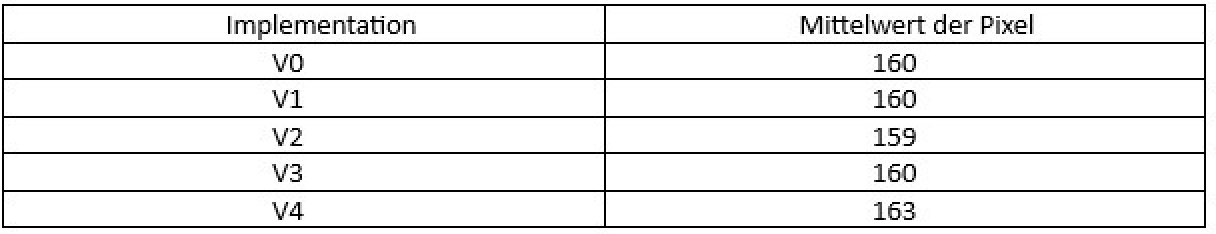
\includegraphics[width = 0.75\textwidth]{images/table.png}
\caption{Berechnung der Mittelwerte mit $\gamma$ = 0.5 und standarte Graustufekoeffizienten}
\label{fig:8}
\end{figure}

Es ist zu erwarten, dass solche Ungenauigkeiten bei Fließkommazahlenberechnungen gibt. Aber jeder Ansatz zeigt die Ausgabedatei klar. Folglich werden zusätzliche Tests zur Zusammenführung verschiedener Parameter beschrieben (mehr dazu in der Performanzanalyse).

\begin{figure}[h]
\centering
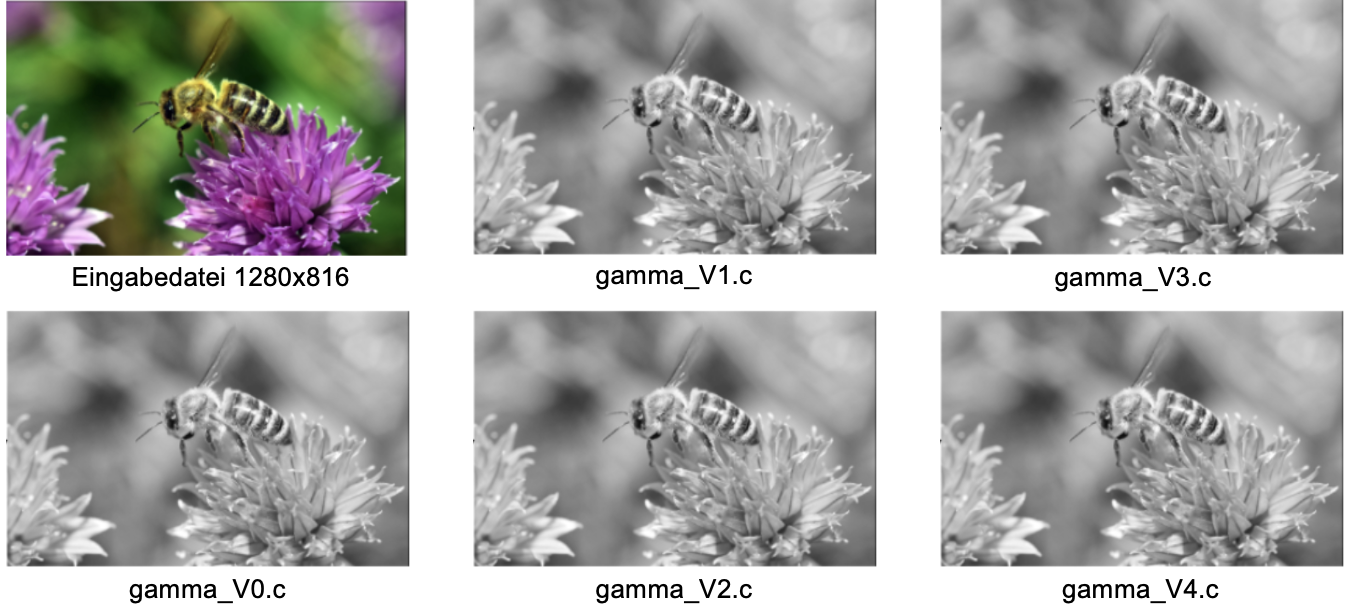
\includegraphics[width = 0.75\textwidth]{images/korrekt_pic.png}
\caption{Die Vergleichung der Ausgabedateien generiert von verschiedenen Implementierungen mit $\gamma$ = 0.5}
\label{fig:7}
\end{figure}

\section{Performanzanalyse}
Um eine Beurteilung der unterschiedlichen Implementierung der Gamma-Korrektur zu treffen, wurde eine Performanzanalyse durchgeführt. Die Analyse umfasst drei Experimente, welche auf unterschiedlichen Bildgrößen sowie Iterationszahlen durchgeführt wurden, um eine umfassende Bewertung der Leistungsfähigkeit der implementierten Version zu ermöglichen.

Das dafür verwendete System mit  Intel Core i7 mit 3,6 GHz, 24 GB DDR4 und Ubuntu 22.04.3 LTS, durchgeführt. Die Softwareumgebung bestand aus  C17 und GCC 11.4.0.

\textbf{1.} \textit{Experiment: ITU-R BT.601-7 (SDTV) mit 680x408 Bild}

Im ersten Experiment wurden die Implementierungen mit einem Standard-Definition-Bild (SDTV) gemäß ITU-R BT.601-7 getestet, und einer Bildgröße von 680x408 Pixel. Die Iterationszahlen variierten von 100 bis 10.000, um die Skalierbarkeit der Implementierungen zu bewerten. Wie in der ersten Grafik ersichtlich, weisen alle Implementierungen zeigen eine lineare Steigerung der Ausführungszeit mit zunehmender Anzahl von Iterationen. Implementierung v1 hat offensichtlich die schlechteste Performance, während v4 die niedrigste Ausführungszeit bei der höchsten Anzahl von Iterationen aufweist. Die vierte Version (v4) eine deutliche Leistungssteigerung gegenüber der Implementierungen v0, v2 und v1, mit einer Reduzierung der Ausführungszeit um ~68\% als v0 und v2 und um 51,46\% als v3, bei 10.000 Iterationen.

\textbf{2.} \textit{Experiment: ITU-R BT.601-7 (SDTV) mit 1920x1224 Bild}

Das zweite Experiment untersuchte die Performanz auf einem größeren Bild von 1920x1224 Pixeln, um die Effekte der Bildgröße auf die Verarbeitungszeit zu analysieren. Die Ergebnisse, dargestellt in der zweiten Grafik, verdeutlichen die Skalierbarkeitsprobleme der Basisimplementierung (v0), insbesondere im Vergleich zu den optimierten Versionen. Version 4 (v4) ist bei größeren Bildern noch überlegener zu den anderen Implementierungen. Im Vergleich ist v4 um das 4.3-fache schneller gegenüber der nächst effizienteren Variante v3, welche ebenfalls eine SIMD Implementation ist. 

\textbf{3.} \textit{Experiment: Durchschnittlicher Pixelwert vs. Gamma-Wert}

Zuletzt wurde der Einfluss verschiedener Gamma-Werte auf den durchschnittlichen Pixelwert untersucht, um die Auswirkungen der Gamma-Korrektur auf die Bildhelligkeit zu quantifizieren. Die Ergebnisse, veranschaulicht in der dritten Grafik, zeigen eine deutliche Abnahme des durchschnittlichen Pixelwerts mit zunehmendem Gamma, was die Effektivität der Gamma-Korrektur bei der Anpassung der Bildhelligkeit bestätigt. \par

\textbf{Zusammenfassung der Experimente} \par
Durch die durchgeführten Experimente konnten wertvolle Erkenntnisse hinsichtlich Leistungsfähigkeit der verschiedenen Implementierungen der Gamma-Korrektur gezeigt werden. Während alle Versionen unter verschiedenen Bedingungen variierende Leistungsniveaus zeigten, hebt sich \textit{v4} als besonders effizient hervor, insbesondere in Bezug auf die Ausführungszeit und Skalierbarkeit. Auch konnte im zweiten Experiment verdeutlicht werden, dass SIMD bei größeren Bildern deutlich effizienter ist als die Basisimplementationen v0 - v2.


\begin{figure}[htbp]
    \centering
    \begin{minipage}{0.45\textwidth}
    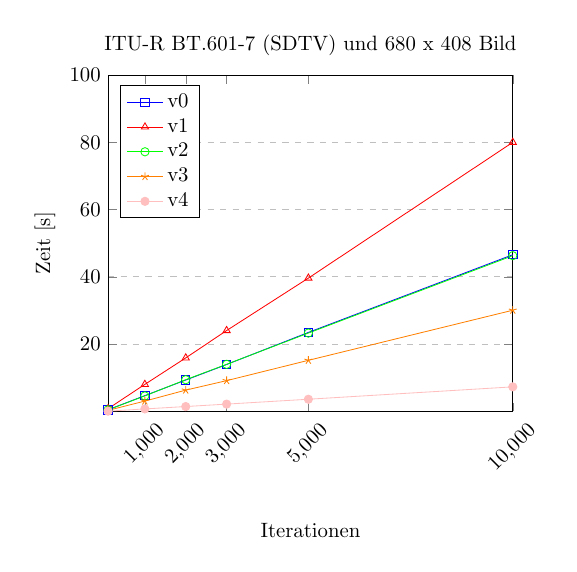
\begin{tikzpicture}[scale=0.75]
    \label{graph:1}
    \begin{axis}[
        title={ITU-R BT.601-7 (SDTV) und 680 x 408 Bild},
        xlabel={Iterationen},
        ylabel={Zeit [s]},
        xmin=100, xmax=10000,
        ymin=0, ymax=100,
        scaled x ticks=false,
        xlabel style={yshift=-1.5em},
        x tick label style={rotate=45},
        xtick={1000,2000,3000,5000,10000},
        ytick={20,40,60,80,100},
        legend pos=north west,
        ymajorgrids=true,
        grid style=dashed,
        cycle list name=color list, % verwendet eine vorgegebene Liste von Farben
    ]
    
    \addplot[
        color=blue,
        mark=square,
        ]
        coordinates {
        (100,0.476928)(1000,4.68402)(2000,9.32)(3000,13.94)(5000,23.48)(10000, 46.59)
        };
        \addlegendentry{v0}
    
    \addplot[
        color=red,
        mark=triangle,
        ]
        coordinates {
        (100,0.8)(1000,8.03)(2000,15.9)(3000,24.04)(5000,39.64)(10000,80.016)
        };
        \addlegendentry{v1}
    
    \addplot[
        color=green,
        mark=o,
        ]
        coordinates {
       (100,0.46)(1000,4.6)(2000,9.42)(3000,13.99)(5000,23.29)(10000, 46.31)
        };
        \addlegendentry{v2}
    
    \addplot[
        color=orange,
        mark=star,
        ]
        coordinates {
        (100,0.31)(1000,3.06)(2000,6.32)(3000,9.14)(5000,15.18)(10000,30.079)
        };
        \addlegendentry{v3}

            \addplot[
        color=pink,
        mark=*,
        ]
        coordinates {
        (100,0.07)(1000,0.725)(2000,1.44)(3000,2.16)(5000,3.61)(10000,7.29)
        };
        \addlegendentry{v4}
        
    \end{axis}
    \end{tikzpicture}

    \end{minipage}\hfill
    \begin{minipage}{0.45\textwidth}
    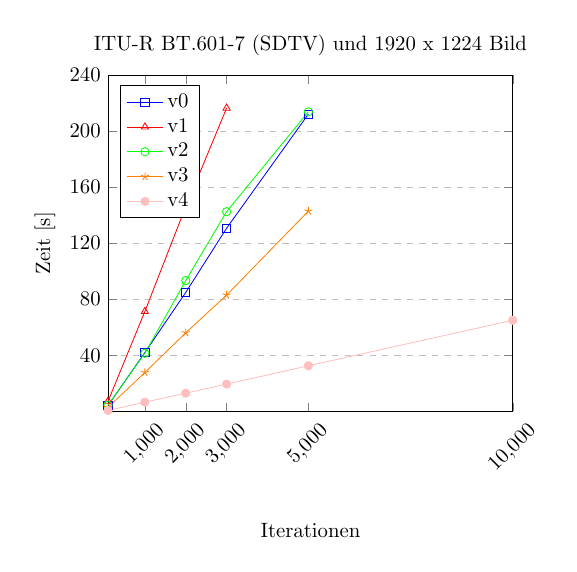
\begin{tikzpicture}[scale=0.75]
    \label{graph:2}
    \begin{axis}[
        title={ITU-R BT.601-7 (SDTV) und 1920 x 1224 Bild},
        xlabel={Iterationen},
        ylabel={Zeit [s]},
        xmin=100, xmax=10000,
        ymin=0, ymax=240,
        scaled x ticks=false,
        xlabel style={yshift=-1.5em},
        x tick label style={rotate=45},
        xtick={1000,2000,3000,5000,10000},
        ytick={40, 80, 120,160,200,240},
        legend pos=north west,
        ymajorgrids=true,
        grid style=dashed,
        cycle list name=color list, % verwendet eine vorgegebene Liste von Farben
    ]
    
    \addplot[
        color=blue,
        mark=square,
        ]
        coordinates {
        (100,4.25)(1000,41.99)(2000,84.88)(3000,130.77)(5000, 212.17)
        };
        \addlegendentry{v0}
    
    \addplot[
        color=red,
        mark=triangle,
        ]
        coordinates {
        (100,7.28)(1000,71.28)(2000,146.11)(3000,216.45)
        };
        \addlegendentry{v1}
    
    \addplot[
        color=green,
        mark=o,
        ]
        coordinates {
       (100,4.5)(1000,41.49)(2000,93.35)(3000,142.55)(5000, 213.82)
        };
        \addlegendentry{v2}
    
    \addplot[
        color=orange,
        mark=star,
        ]
        coordinates {
        (100,2.82)(1000,27.75)(2000,56.09)(3000,83.00)(5000,142.95)
    
        };
        \addlegendentry{v3}
    \addplot[
        color=pink,
        mark=*,
        ]
        coordinates {
        (100,0.64)(1000,6.56)(2000,12.98)(3000,19.46)(5000,32.54)(10000, 65.04)
        };
        \addlegendentry{v4}
    \end{axis}
    \end{tikzpicture}
    \end{minipage}
\end{figure}
    
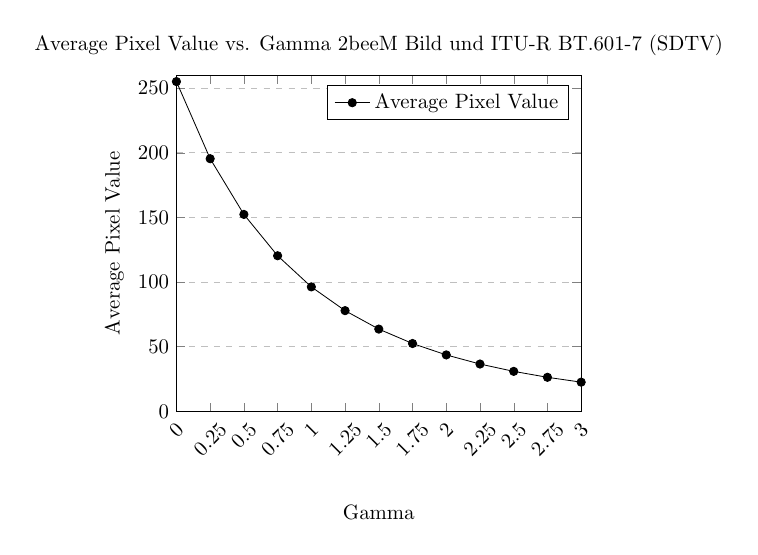
\begin{tikzpicture}[scale=0.75]
\centering
\label{graph:3}
\begin{axis}[
    title={Average Pixel Value vs. Gamma 2beeM Bild und ITU-R BT.601-7 (SDTV)},
    xlabel={Gamma},
    ylabel={Average Pixel Value},
    xmin=0, xmax=3,
    ymin=0, ymax=260,
    xlabel style={yshift=-1.5em},
    x tick label style={rotate=45},
    xtick={0,0.25,...,3},
    ytick={0,50,...,250},
    legend pos=north east,
    ymajorgrids=true,
    grid style=dashed,
]

\addplot[mark=*,black] coordinates {
    (0.00,255.00) (0.25,195.37) (0.50,152.29) (0.75,120.33) (1.00,96.26) (1.25,77.88) 
    (1.50,63.62) (1.75,52.47) (2.00,43.65) (2.25,36.60) (2.50,30.93) (2.75,26.34) (3.00,22.58)
};
\legend{Average Pixel Value}
\end{axis}
\end{tikzpicture}

\section{Zusammenfassung und Ausblick}
In dieser Arbeit wurde die Anwendung der Gamma-Korrektur auf Bilder im 24bpp PPM-Format in Graustufen umgewandelt und anschließend mittels Gamma-Korrektur in Helligkeit und Kontrast angepasst wurden. Die Analyse von vier Implementierungsansätzen in C hat gezeigt, dass trotz unterschiedlicher Methoden keine signifikanten Leistungsunterschiede zwischen den skalar basierten Versionen (v0 und v3) festgestellt wurden. Die Untersuchung hebt das Potenzial von SIMD-Parallelismus zur Leistungssteigerung hervor.

Für zukünftige Arbeiten könnte die Erkundung von SIMD-Optimierungen und adaptiven Gamma-Korrekturtechniken weitere Verbesserungen in Effizienz und Anpassungsfähigkeit an unterschiedliche Bildinhalte bieten. Dies könnte unter anderem durch eine Implementierung von Parallel Computing erreicht werden, vor allem in Kombination mit SIMD.

% TODO: Fuegen Sie Ihre Quellen der Datei Ausarbeitung.bib hinzu
% Referenzieren Sie diese dann mit \cite{}.
% Beispiel: CR2 ist ein Register der x86-Architektur~\cite{intel2017man}.
\bibliographystyle{plain}
\bibliography{Ausarbeitung}{}

\end{document}
